\documentclass[a4paper, 12pt]{article}
\usepackage[a4paper,textwidth=170mm,textheight=245mm]{geometry}

\usepackage[utf8]{inputenc}
\usepackage{todonotes}
\usepackage{amsmath}
\usepackage{parskip}
\usepackage{listings}
\usepackage{float}
\usepackage{url}
\usepackage{hyperref}

% For the wrapfigure
\usepackage{wrapfig}
\usepackage{caption}
\usepackage{subcaption}
\usepackage{color, colortbl}

\definecolor{Green}{rgb}{0.23,0.72,0.16}

\begin{document}
\date{}

\title{\Large Classy: Feature Evaluation using Naive Bayes for Genre Classification}

\author{
{Michael Sörsäter}\\
IDA Linköping
}

\maketitle

% Use the following at camera-ready time to suppress page numbers.
% Comment it out when you first submit the paper for review.
%\thispagestyle{empty}

\subsection*{Abstract}
Your Abstract Text Goes Here.  Just a few facts.
Whet our appetites.

\section{Introduction}
Music is a big part of our modern society.
According to Spotify, during 2017 I personally listened to over 60 000 minutes of music. \cite{spotify}
As everything else in our world we order things and place them in different categories.

Music is often categorized in large genres like \textit{pop}, \textit{rap} and \textit{rock} and is in turn categorized further, like \textit{indiepop}, \textit{dream pop} and \textit{synth pop}.
The most defining features of a genre is the sound, which instruments is used, the tempo, and the structure of the song like number of Verses and Choruses.
Even if the sound have the greatest impact when deciding a genre the lyrics tend to follow certain patterns.

I think that pop music generally tend to be about love and easier subjects whereas rap usually have more complex language and have a more storytelling structure.

In this project a classifier will be implemented to determine the genre of songs.
Different features will be considered to classify the genres and will be evaluated to see if they improve the result or not.
A lot of focus will lie on comparing the two genres pop and rock but also on all 6 genres.

\section{Teory}
The Naive Bayes classifier is commonly used for music classification and have shown in previous work to be an effective model for document classification. \cite{Canicatti}

\subsection{Naive Bayes}
Naive Bayes build a probabilistic model that uses arbitrary features from documents.
When training the model features are extracted for different documents and are feeded to the model together with the document class.
For each feature and class the probability in formula \ref{eq:feat} is calculated where $ feat_{i}$ is feature i and $ class_k $ is class k.

\large
\begin{equation}
    p (feat_{i}|class_{k})
    \label{eq:feat}
\end{equation}
\normalsize

When predicting the class of a document the same features are extracted and given to formula \ref{eq:bayes} where there exist $K$ classes and $n$ features for each document.
The probability of the class is multiplied by all features explained in formula \ref{eq:feat}.
The predicted class is the one with highest probability.

\large
\begin{equation}
    \hat{y} = \underset{k \in \{1,2,...,K\}}{argmax} \, \, \, p(class_{k}) \prod_{i=1}^{n} p (feat_{i}|class_{k}
    \label{eq:bayes}
\end{equation}
\normalsize

The strength of the Naive Bayes classifier is that the features are arbitrary.
The model determine the importance for all features and let informative features influence the prediction a lot as well as assign uninformative features with low probabilities.danc

\section{Data set}
\label{sec:dataset}
The acquisition of a good data set is a task that requires careful consideration.
Usually one artist (will use the word artist for artist/band/group) are labeled with just one genre and all songs produced by that artist are assumed to be that genre. \todo{länka till det fam}
This assumption can result in a lot of bad classification as one artist is not bound to one genre.
Previous obtained data sets were considered.
The problem with copywriting often have the impact that bag of words model are used where the different words are coverted to integers. \todo{ref-million song dataset}
This representation makes it hard to work with the models and to evaluate the result.
Many data sets found had not been classified with genres or had to many genre classes in them.
For these reason I made the decision to create my own corpus.

When the data set was created three steps were followed.
Firstly, getting lists of tracks tagged with their genre.
Secondly, from the name of the tracks, get an url to a webpage hosting lyrics.
Thirdly, from the urls, scrape and store the lyrics.

\subsection{List of tracks}
Across the internet it exist a lot of different lists of songs in different genres.
The following criterias were considered when looking for lists of tracks:
\begin{itemize}
    \item {\textbf{Organization} - lists made by individuals can be subjective and is avoided. Lists by organizations tend to be more thought through.}
    \item {\textbf{Reliable} - the producer behind the list should have a lot of experience and knowledge about music.}
    \item {\textbf{Genre cover} - the different genres should come from the same source. Many lists of just \textit{rap} or \textit{electronic} exist but are produced by different persons/organizations.}
    \item {\textbf{Few genres} - because of limitations in the project scope and computational power just a few genres should be included. The goal was to have at top around 5 different genres.}
    \item {\textbf{A lot of data} - to get a reliable model at least a couple of hundred songs is needed in each genre}
\end{itemize}

I found that billboard fulfills all these criterias.

Billboard is a music magazine that was founded in 1894.
Since then billboard have been an important organization in the music industry.
Each year they release lists of the topmost tracks in different categories.
Among other lists they have lists for the genres \textit{pop}, \textit{country}, \textit{rock}, \textit{r\&b/hip-hop}, \textit{rap} and \textit{dance/electronic}. \cite{billboard}

For the different lists, there is data from the latest 5-10 years which makes a decent amount.
By going through these webpages with lists and scraping the data the corpus was created.

%Some lists were missing so I used Wayback Machine \todo{länka till det kanske?} to retrieve some data and also found a missing list in a forum.

Each genre have a lot of different lists and the number of lists were chosen to try to get an even distribution between the genres. For rock, it was sufficient to just use one list but for rap, all available lists were used.
The genres used are shown together with the name of the lists.
\begin{itemize}
    \item {\textbf{Pop} - Uses the lists: ``pop'', ``adult pop'', ``adult contemporary''}
    \item {\textbf{Rap} - Uses the lists: ``hot rap'', ``rap streaming'', ``rap airplay'', ``rap digital''}
    \item {\textbf{Rock} - Uses the lists: ``hot rock''}
    \item {\textbf{Electronic} - Uses the lists: ``hot dance electronic''}
    \item {\textbf{Country} - Uses the lists: ``hot country''}
    \item {\textbf{R\&b} - Is a combination of the genres r\&b and hip-hop. Mostly focuses on r\&b. Uses the lists: ``hot r\&b'', ``r\&b streaming'', ``hot r\&b and hip-hop'', ``r\&b and hip-hop streaming'', ``r\&b and hip-hop airplay''}
\end{itemize}

From the lists the name of the artist, song and genre were saved and duplicates were removed.
If there existed several copies within the same genre only one was saved.
Duplicates within the same genre comes from that many lists are similar to each other or that songs are on top lists for multiple years.
If one song was labeled with more than one genre, all occurences of that song were removed.
From all lists the total number of songs were around 6000.
After removing duplicates within the same genre around 4200 remained and after removing songs in more than one genre 3271 were left.

The tracks are saved in a json file with key an integer counter and value artist, title and genre.

\subsection{Match tracks with urls}
From the name of the tracks the Genius API was used to find the urls. \cite{genius}

Using the API a search query was sent with the artist and title in it.
The API returned the matches for the search query.
If the artist and title had an exact match the url was returned.

During this process there were a lot of variantions on the spelling so if the Levenshtein distance between the names were less than 2 they were considered a match.
For the tracks that didn't have a match, the alternatives the search query returned were given to the user.
By entering the index for the correct alternative the url was returned.

For some tracks the Genius API didn't found the correct song and for these the urls were found by hand.

The linking between track and url is made in a separate json file which makes it possible to use another project file where the tracks belong to other genres.

\subsection{Scrape lyrics}
From the json file with the tracks and urls all urls were retrieved from Genius.
Their API does not support to get the lyrics so regular scraping was used with \textit{requests} and \textit{Beautiful Soup}. \cite{requests} \cite{bs4}
The lyrics was stored in files named artist + title.
Of all songs, the lyrics was not available for 5 of them so they were removed from the project file, reducing the number of songs from 3271 to 3266.

The songs sorted by genre can be found in table \ref{tab:distribution}.
\begin{table}[h]
    \begin{center}
        \begin{tabular}{| l | r |}
            \hline
            Genre & Count \\ \hline
            all & 3266 \\
            pop & 700 \\
            rap & 322 \\
            rock & 613 \\
            electronic & 389 \\
            country & 423 \\
            r\&b & 824 \\ \hline
        \end{tabular}
        \caption{Genre distribution in corpus}
        \label{tab:distribution}
    \end{center}
    \end{table}

\section{Method}
As mentioned in section \ref{sec:dataset} the data set was created by scraping lyrics from Genius by using lists obtained from billboard.

When the data was in place the classifier was created.
The library nltk for Python3 was used in this project. \cite{nltk}
For the classifier, a class was created that is based on the class ``NaiveBayesClassifier'' found in nltk.

When running the classifier a project file is required.
From the project file the corpus is created.
The corpus exist of the lyrics together with the true genre.
When the corpus is created it is shuffled.
The seed for the random function is initialized with a constant value to ensure reproducibility.

\subsection{Baseline}
\label{sec:baseline}
The classifier is initialized with the shuffled corpus and the data is split up in train data and test data.
The default values are that $70\%$ are train and $30\%$ are test data.
Preprocessing of the training data is made to extract all unigrams.
For each song, each line are split by a space and the words are saved.
The most common unigrams are found by sorting all unigrams by their frequencies and the topmost 2500 are stored.

For each song in both the training data and test data the unigrams are extracted in the same way as in the preprocessing phase.
Each song will have boolean unigram features if the unigrams exist in the most common features or not.

The model is trained by the features in the train data and tested with the features in the test data.
The accuracy is calculated for the test set.
For each genre the precision, recall and f-measure is derived.

\subsection{Features}
\label{sec:feat}
In the classifier several features are added and explained in this section.

\subsubsection*{Unigram threshold}
When using all data, the maximum number of unigram features are around 37000 but with so many features the system takes really long to run, it fills up my personal RAM-memory, and the performance is only marginally better.
Any unigram must be seen atleast two times in the training data to be included in the model which reduces the number of unigram features to around 19000.
The default value is set to 2500.

\subsubsection*{N-gram and n-gram threshold}
In the model bigrams, trigrams, four-grams and five-grams are implemented.
They are extracted in the same way as the unigrams.
The number of n-grams used in the model are settable parametes with the default value set to 2000 for bigrams, 3000 for trigrams, 1000 for four-grams and 1000 for five-grams.

\subsubsection*{Meta data}
The lyrics found at Genius sometimes contain metadata about the structure of the songs.
One example is the song \textit{Ed Sherran - Thinking Out Loud}: \cite{ed_thinking}

\begin{verbatim}
    [Verse 1]
    When your legs don't work like they used to before
    And I can't sweep you off of your feet
    ...

    [Pre-Chorus 1]
    People fall in love in mysterious ways
    Maybe just the touch of a hand
    ...

    [Chorus]
    So honey, now, take me into your loving arms
    Kiss me under the light of a thousand stars
    ...

    [Verse 2]
    ...

    [Pre-Chorus 2]
    ...

    [Chorus]
    ...

    [Chorus]
    ...

\end{verbatim}

This structure, \textit{verse}, \textit{chorus}, \textit{verse}, \textit{chorus}, \textit{chorus} is a typical structure for a pop song.
Other types that are used in the model: \textit{intro}, \textit{outro}, \textit{break}, \textit{bridge}, \textit{skit}, \textit{hook}, \textit{drop}, \textit{interlude} and \textit{breakdown}.
When processing lyrics to extract n-grams the lines that starts and ends with ``[ ]'' are ignored to avoid adding these words to the model.
When the features metadata is added the classifier looks for the types within the brackets.
The number for each type is added as the feature.

\subsubsection*{Word editing}
Three features are added to handle the interpretation and editing of the lyrics.
\begin{enumerate}
    \item {\textbf{Stopwords} - With this feature all stopwords are ignored.
    Stopwords are words that often are the same, independent of the genre.
    The stopwords used are the ones found in the nltk library and items in pythons' punctuation found in the library string.}
    \item {\textbf{Tokenization} - Usually tokenization is made at the beginning when processing documents.
    In this baseline system the tokenization is made by hand, as explained in section \ref{sec:baseline}.
    This feature utilizes the word tokenization found in nltk instead of manual tokenization.}
    \item {\textbf{Stemming} - In regular text many words are inflected and the basic word, stem, is often the wanted word.
    This feature uses the nltk SnowballStemmer to stem the words.}
\end{enumerate}

\subsubsection*{Length of lyrics}
The length of the lyrics can be an indication on the genre.
Some electronic songs are usually short and repetative with many parts in the song just music.
Hip\/hop and rap are previously shown to contain longer lyrics and more complex language. \cite{rap-long}

Three features were added:
\begin{itemize}
    \item {Number of characters}
    \item {Number of words}
    \item {Number of unique words}
\end{itemize}

The features are boolean features.
The feature takes a threshold value that determines the value of the feature.
Finding threshold values are tricky, especially when all genres are included, the difference can be small between too many genres.
When analyzing the counts, normalized histograms are created that are colored by genre.
Figure \ref{fig:words} shows the number of words in all pop and rap songs and the number of characters in all genres.
In \textit{a} the difference between the genres are significant in relation to the messy distribution of the number of characters with all genres in \textit{b}.

\begin{figure}[H]
    \centering
    \begin{subfigure}[b]{0.48\textwidth}
        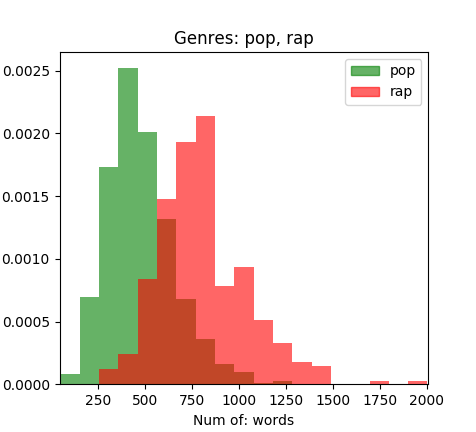
\includegraphics[width=\textwidth]{res/words-pop_rap.png}
        \caption{Number of words in pop and rap}
    \end{subfigure}
    ~ % spacing
    \begin{subfigure}[b]{0.48\textwidth}
        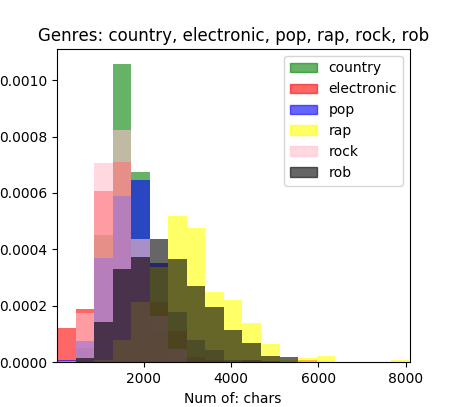
\includegraphics[width=\textwidth]{res/chars-country_electronic_pop_rap_rock_rob.png}
        \caption{Number of characters in all genres}
    \end{subfigure}
    \caption{Length of lyrics}
    \label{fig:words}
\end{figure}

\subsection{Options}
To run and use the system several options are added to the system which are exlained below.

\begin{itemize}
    \item {\textbf{Genres} - Default is to use all genres but can can be changed to any genres that are provided in the project file.
    When testing certain features it is only relevant to have a few number of genres.}
    \item {\textbf{Iterations} - When running a test the data is shuffled and then split up in train and test.
    Between different runs the result can differ so to get reliable result the test need to be run a number of times.
    The number of iterations are determined by this option.}
    \item {\textbf{Split} - In the baseline system the default value to split training and test data is 70 and 30 percent respectively.
    This can be changed with the parameter split.}
    \item {\textbf{Count} - Default is to use all songs in each genre. With this option the number of songs is limited to the provided argument. Makes testing system quicker.}
    \item {\textbf{Show features} - Provided with a value n. Shows the n most informative features in the model.}
    \item {\textbf{Stats} - Show precision, recall and f-measure for the model.}
\end{itemize}

\subsection{Code}
During this project a lot of effort was made in making a good and usable system, for both scraping, getting lyrics, use different features and run different tests.
The code can be found at github. \cite{github}
Documentation on how to run the system can be found in the repository's ``README''.

\section{Results}
The results will focus mainly on comparing two different genres or comparing all genres.
For all results the split in train and test is 70\% and 30\% respectively and all tests have been running for 5 iterations.
All other arguments use the default values.
Between different tests the random seed is reseted which makes the results reproducible.

Performance for the baseline system is shown in table \ref{tab:res-baseline}.

\begin{table}[h]
\begin{center}
    \begin{tabular}{| l | r |}
        \hline
        Genres & Accuracy \\
        \hline
        all 6 genres & 53.20 \% \\
        pop and rap & 93.22 \% \\
        \hline
    \end{tabular}
    \caption{Accuracy of baseline system}
    \label{tab:res-baseline}
\end{center}
\end{table}

\subsection{Unigrams}
\label{sec:unigrams}
The threshold value for the unigrams are examined for a number of values and shown in table \ref{tab:res-uni}.
When using few features stopwords can make a big difference so each test is also tried by ignoring stopwords.

\begin{table}[h]
\begin{center}
    \begin{tabular}{| r | r | r |}
        \hline
        \# of features & Accuracy & Stopwords \\
        \hline
        10  & 33.82 \% & 36.37 \% \\
        50  & 42.59 \% & 43.92 \% \\
        100  & 46.24 \% & 46.49 \% \\
        500  & 50.31 \% & 51.02 \% \\
        1000  & 52.20 \% & 52.47 \% \\
        2500 (default)  & 53.20 \% & 52.35 \% \\
        10000  & 54.16 \% & 52.49 \% \\
        \hline
    \end{tabular}
    \caption{Accuracy for unigrams thresholds, normal and ignoring stopwords}
    \label{tab:res-uni}
\end{center}
\end{table}

\subsection{N-grams}
The different n-grams are examined both individually, without unigrams and together with each other.
For all tests the threshold values are as defined in \ref{sec:feat}, unigram 2500, bigram 2000, trigram 3000 and 1000 for four-gram and five-gram.
The tests are shown in table \ref{tab:res-ngram}.
The first line is the baseline system, every test that performs better than that is marked green.

\begin{table}[h]
\begin{center}
    \begin{tabular}{| r | r | r | r | r | r |}
        \hline
        Unigram & Bigram & Trigram & Four-gram & Five-gram & Accuracy \\
        \hline
        % Unigram
        1 &   &   &   &   & 53.20 \% \\ \hline
        % Bigram
          & 1 &   &   &   & 47.76 \% \\ \hline
        \rowcolor{Green}
        1 & 1 &   &   &   & 54.16 \% \\ \hline
        % Trigram
          &   & 1 &   &   & 38.02 \% \\ \hline
        \rowcolor{Green}
        1 &   & 1 &   &   & 53.59 \% \\ \hline
        \rowcolor{Green}
        1 & 1 & 1 &   &   & 53.49 \% \\ \hline
        % Fourgram
          &   &   & 1 &   & 29.96 \% \\ \hline
        \rowcolor{Green}
        1 &   &   & 1 &   & 54.25 \% \\ \hline
        \rowcolor{Green}
        1 & 1 & 1 & 1 &   & 53.27 \% \\ \hline
        % Five-gram
          &   &   &   & 1 & 23.90 \% \\ \hline
        \rowcolor{Green}
        1 &   &   &   & 1 & 54.10 \% \\ \hline
        1 & 1 & 1 & 1 & 1 & 52.88 \% \\ \hline
    \end{tabular}
    \caption{Accuracy n-grams}
    \label{tab:res-ngram}
\end{center}
\end{table}

\subsection{Meta data}
The performance when adding the feature about meta data is shown in table \ref{tab:res-meta}.
Different tests are made with varying number of genres.
The accuracy is calculated by using the baseline system and then adding the feature.

\begin{table}[h]
\begin{center}
    \begin{tabular}{| r | r | r |}
        \hline
        Genres & Normal & Meta Data \\
        \hline
        All genres & 53.20 \% & 54.49 \% \\

        pop, rap & 93.22 \% & 93.29 \% \\

        country, rap & 97.05 \% & 97.41 \% \\

        electronic, rock & 75.47 \% & 77.53 \% \\

        electronic, r\&b & 82.15 \% & 82.20 \% \\
        \hline
    \end{tabular}
    \caption{Accuracy for meta data feature}
    \label{tab:res-meta}
\end{center}
\end{table}

\subsection{Word editing}
The three different word types are tested on all genres and on the genres \textit{pop} and \textit{rap}.
Results from the word editing are found in table \ref{tab:res-words}.

\begin{table}[h]
\begin{center}
    \begin{tabular}{| l | l | l | r | r | }
        \hline
        Stopwords & Tokenize & Stem & Acc (pop rap) & Acc (all) \\
        \hline
          &   &   & 93.22 \% & 53.20 \% \\ \hline
        1 &   &   & 93.09 \% & 52.35 \% \\ \hline
          & 1 &   & 93.09 \% & 51.90 \% \\ \hline
          &   & 1 & 93.22 \% & 52.59 \% \\ \hline
        1 & 1 &   & 93.22 \% & 51.57 \% \\ \hline
        1 &   & 1 & 93.09 \% & 52.76 \% \\ \hline
          & 1 & 1 & 93.42 \% & 51.76 \% \\ \hline
        1 & 1 & 1 & 93.22 \% & 53.20 \% \\ \hline
    \end{tabular}
    \caption{Accuracy for word features}
    \label{tab:res-words}
\end{center}
\end{table}

\subsection{Length of lyrics}
Using information about length of lyrics is tested and the result is shown in table \ref{tab:res-lengths}.

\begin{table}[h]
\begin{center}
    \begin{tabular}{| l | l | l | r | r |}
        \hline
        Genres & Type (\# of)& Threshold & Acc (normal) & Acc (feature) \\
        \hline
        all             & characters    & 2000 & 53.20 \% & 53.20 \% \\ \hline
        electronic, pop & characters    & 2000 & 76.32 \% & 76.32 \% \\ \hline
        all             & words         & 600  & 53.20 \% & 53.25 \% \\ \hline
        country, rap    & words         & 600  & 97.05 \% & 97.32 \% \\ \hline
        all             & unique words  & 100  & 53.20 \% & 53.18 \% \\ \hline
        rock, r\&b      & unique words  & 100  & 88.57 \% & 88.70 \% \\ \hline
    \end{tabular}
    \caption{Accuracy for normal model and with feature added}
    \label{tab:res-lengths}
\end{center}
\end{table}

\subsection{Statistics}
For all tests the accuracy have been the measure of choice.
The accuracy is easy to compare to each other but have limitations.
The precision, recall and f-measure for the tests are available and some results from that will be presented.

During the project the genres \textit{pop} and \textit{rap} have been the main focus.
For those two genres, 1 iteration give the accuracy $93.16\%$.
The other measures are shown in the first 2 rows in table \ref{tab:res-stats1}.

When comparing only two genres, the best result is acheived for the two genres \textit{country} and \textit{rap}. The accuracy for that test is $95.98\%$ and the other measures are shown in the last two lines in table \ref{tab:res-stats1}.

The same test is done for the genres \textit{country} and \textit{rap}, with the accuracy $95.98\%$ and are shown in the two last lines.

\begin{table}[h]
\begin{center}
    \begin{tabular}{| l | r | r | r |}
        \hline
        Genre & Precision & Recall & F-measure \\
        \hline
        pop     & 95.77 \% & 94.44 \% & 95.10 \% \\ \hline
        rap     & 87.23 \% & 90.11 \% & 88.65 \% \\ \hline
                &          &          &          \\ \hline
        country & 93.23 \% & 100.00\% & 96.50 \% \\ \hline
        rap     & 100.00\% & 91.00 \% & 95.29 \% \\ \hline
    \end{tabular}
    \caption{Accuracy for normal model and with feature added}
    \label{tab:res-stats1}
\end{center}
\end{table}

\section{Discussion}
When comparing all genres, the accuracy is $53.20 \%$.
This data set is new so the result can't be compared to old results.
With 6 genres, by just guessing, the accuracy would be $16.67 \%$ so compared to that it seems to be alright.

The two genres I was most interested in was \textit{pop} and \textit{rap}.
The classifier performs well to make a difference between the two, the accuracy was $93.22 \%$.
Rap tends to contain a lot of curses and in general, bad language.
The 10 most informative features when comparing the two genres are listed together with the ratio, rap:pop.

\begin{enumerate}
    \item{``Fuck'' - 66:1}
    \item{``bitches'' - 59:1}
    \item{``nigga'' - 44:1}
    \item{``niggas'' - 41:1}
    \item{``bitch'' - 39:1}
    \item{``rich'' - 38:1}
    \item{``fucked'' - 36:1}
    \item{``shit'' - 31:1}
    \item{``ho'' - 29:1}
    \item{``Nigga'' - 29:1}
\end{enumerate}

So, to write a rap song, use a lot of curses.

\subsection{Unigrams}
A lot of information is found in very few features.
When using so few features, it is necessary to remove the stopwords.
With only 100 features and removing stopwords the accuracy ($46.49\%$) is $87.39\%$ of the baseline value ($53.20\%$).

\subsection{N-grams}
When analyzing the n-grams the most information is found in the unigrams.
No n-gram alone performed better than them, but all additions of a n-gram (except last with all n-grams added) improves the accuracy.
I realized that the four-grams and five-grams quickly became bad, it was mostly repetions of words like ``la, la, la, la, la''.
With to long n-grams it is hard to match anything else than that exact song it appears in.

\subsection{Meta data}
In all examples tried, the feature about meta data made an inprovement.
The increased accuracy was not of great magnitude but still an increase.
The count of the number of types is a hint on the correct genre.

\subsection{Word editing}
For the two genres \textit{pop} and \textit{rap}, adding the word features didn't make a big impact on the result.
Out of 7 tests, 3 performed the same, 3 performed slightly worse and 1 performed slightly better.
Removing stopwords will probably not make a big difference when 2500 unigram features are considered.
More interesting result are found when removing stopwords with few unigram features, shown in section \ref{sec:unigrams}

\subsection{Length of lyrics}
The difference in performance for all genres is marginal, the result doesn't change at all.
As shown in figure \ref{fig:words} part \textit{b}, everything is very messy.
To find differences between genres it is necessary to compare genres that vary.
Country and rap differ a lot, which give an $0.27\%$ increase.
It's not a huge difference, but it still made an impact.
\subsection{Statistics}
% What do you make of it? Discuss your results and
% present your analysis in terms of the background theory.
A rule of thumb is that by considering more unigram features the performance increases a lot.
But, with just few features the classifier performs well.
\section{Conclusion}
The project tried to find features that with an hypothesis behind it, could improve the performance of the Naive Bayes classifier.

The classifier performed, in some situations, better than the baseline system.
This must be considered that the project succeeded, it was possible to find feature that inproved the performance.

I learned that a lot from this project.
% In what sense has your project reached its goal?
% What did you learn from your project?

\section*{References}
% Present a complete list of references.
% Choose a bibliographic style and stick to it.

\bibliographystyle{ieeetr}
\bibliography{res/classy}

\end{document}

